\documentclass[11pt]{article}

\usepackage[margin=1in]{geometry}
\usepackage{amsmath,amssymb,bm}
\usepackage{tikz}
\usepackage{xcolor}
\usepackage{booktabs}
\usepackage{multirow}
\usepackage[colorlinks=true,linkcolor=blue!55!black]{hyperref}

\usetikzlibrary{arrows.meta,positioning,calc,decorations.pathmorphing,
                patterns,backgrounds,fit}

\definecolor{darkfam}{RGB}{197,90,17}
\definecolor{brightfam}{RGB}{31,102,160}
\definecolor{softc}{RGB}{176,42,55}
\definecolor{phot}{RGB}{60,60,140}
\definecolor{gsc}{RGB}{90,90,90}
\definecolor{acc}{RGB}{20,130,90}

\newcommand{\bq}{\bm q}
\newcommand{\Wp}{W_p}
\newcommand{\Wpd}{W_p^{\dagger}}

\title{\bfseries Why the zone-boundary mode is soft\\[2pt]
\large A microscopic account of the $L$-point excitation in the
pyrochlore ring-exchange model}
\author{}
\date{}

\begin{document}
\maketitle
\vspace{-3.2em}

\begin{center}
\begin{minipage}{0.9\textwidth}\small\itshape
This note explains, from the bottom up, why one excitation at the
zone-boundary $L$ point costs half of what its partner at the same
momentum costs. The whole argument rests on one identity: in the ice
basis the neutron probe is a \emph{diagonal} operator, so a ring
exchange either changes the value it reads or it does not. Everything
else follows.
\end{minipage}
\end{center}

\vspace{0.8em}

\section{The one thing to remember about the energy}

The model is the pure ring-exchange Hamiltonian on the spin-ice
manifold,
\begin{equation}
H=-K\sum_p\bigl(\Wp+\Wpd\bigr),
\qquad
\Wp=S^+_1S^-_2S^+_3S^-_4S^+_5S^-_6 ,
\label{eq:H}
\end{equation}
where $p$ runs over the elementary hexagons of the pyrochlore lattice.
$\Wp$ takes an ice configuration in which the six spins around $p$
alternate up--down--up--down--up--down and flips all six at once.

Equation~(\ref{eq:H}) has no diagonal part. There is no potential
energy, no field term, nothing but resonance. The immediate consequence
is the only fact about energy we will need:

\begin{center}
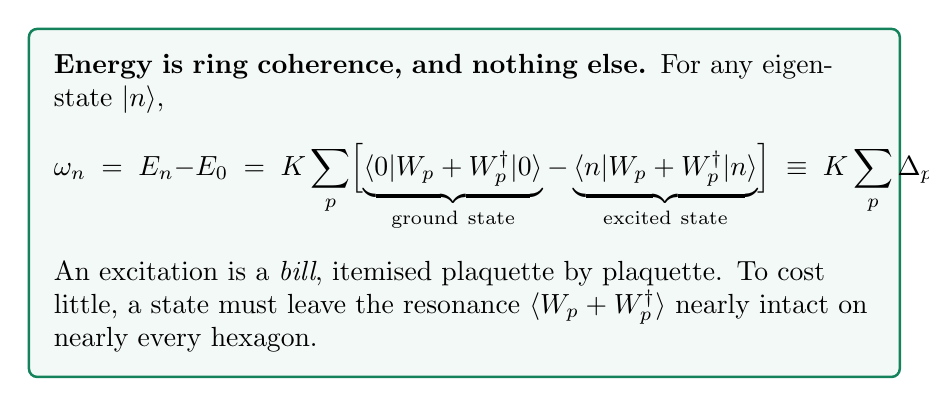
\begin{tikzpicture}
\node[draw=acc,line width=0.9pt,rounded corners=3pt,inner sep=9pt,
      fill=acc!5,text width=0.86\textwidth]{
\textbf{Energy is ring coherence, and nothing else.} For any eigenstate
$|n\rangle$,
\[
\omega_n \;=\; E_n-E_0
\;=\; K\sum_p\Bigl[\underbrace{\langle 0|\Wp+\Wpd|0\rangle}_{\text{ground state}}
-\underbrace{\langle n|\Wp+\Wpd|n\rangle}_{\text{excited state}}\Bigr]
\;\equiv\; K\sum_p\Delta_p(n).
\]
An excitation is a \emph{bill}, itemised plaquette by plaquette. To cost
little, a state must leave the resonance $\langle\Wp+\Wpd\rangle$ nearly
intact on nearly every hexagon.};
\end{tikzpicture}
\end{center}

\noindent
This is exact and additive, and at $48$ sites we can read off every line
of the bill from the exact eigenvector. That is what makes the question
``why is this state cheap?'' answerable rather than rhetorical.

\section{In the ice basis the probe is diagonal}

The emergent electric field is the spin itself, $E_\ell=S^z_\ell$, so
the operator that neutrons couple to is
\begin{equation}
A^\mu_{\bq}=\sum_{i\in\mu}e^{-i\bq\cdot\bm r_i}S^z_i ,
\label{eq:probe}
\end{equation}
one operator for each of the four pyrochlore sublattices $\mu$. (The
response $S^{zz}$ sums $|\langle n|A^\mu_{\bq}|0\rangle|^2$ over $\mu$;
the sublattice label matters, and we will see in
\S\ref{sec:caveat} what goes wrong if it is dropped.)

Now the key structural point. We work in the basis of ice
configurations $|c\rangle$. In that basis $S^z_i$ is diagonal, so
$A^\mu_{\bq}$ is \emph{diagonal too}:
\begin{equation}
A^\mu_{\bq}|c\rangle=a^\mu(c)\,|c\rangle,
\qquad
a^\mu(c)=\sum_{i\in\mu}e^{-i\bq\cdot\bm r_i}S^z_i(c).
\label{eq:diag}
\end{equation}
Each configuration carries a single complex number $a^\mu(c)$: the
amplitude of the imposed density wave in that configuration.

The ring exchange, by contrast, is purely off-diagonal: it takes
$|c\rangle$ to $|c'\rangle$ with hexagon $p$ flipped. So we can ask a
completely concrete question:

\begin{center}
\emph{when a ring exchange moves the system from $c$ to $c'$, does the
number the probe reads change?}
\end{center}

Because only six spins move, the answer is a short computation, and it
is the commutator $[A^\mu_{\bq},\Wp]=g^\mu_p(\bq)\Wp$ written as a
statement about configurations:
\begin{equation}
\boxed{\;a^\mu(c')-a^\mu(c)=\pm\,g^\mu_p(\bq)\;}
\qquad
g^\mu_p(\bq)=\!\!\sum_{j\in p\,\cap\,\mu}\!\!(-1)^{j}
e^{-i\bq\cdot\bm r_j}.
\label{eq:shift}
\end{equation}
The quantity $g^\mu_p$ --- the alternating lattice curl of the imposed
wave around plaquette $p$ --- is \emph{exactly the amount by which
flipping $p$ shifts the density-wave amplitude}. We verified
Eq.~(\ref{eq:shift}) directly on $4000$ ice configurations, every
hexagon, every sublattice: the largest discrepancy was
$0.000\times10^{0}$.

\section{Geometry: some plaquettes are blind to the wave}

Equation~(\ref{eq:shift}) turns a dynamical question into a geometric
one. When is $g^\mu_p=0$?

A pyrochlore hexagon is planar, and its plane is perpendicular to one of
the four $\langle111\rangle$ axes. Each hexagon omits exactly one
sublattice, and that omitted label $\mu$ names its axis, so the hexagons
fall into four \emph{families} of equal size (twelve each on our
$48$-site cluster).

A plane wave $e^{-i\bq\cdot\bm r}$ is constant on planes perpendicular
to $\bq$ --- its wavefronts. So if a hexagon's plane \emph{is} a
wavefront, all six of its sites carry the same phase, the alternating
sum cancels term by term, and $g^\mu_p=0$ for every $\mu$. That happens
precisely when $\bq$ is parallel to that family's $\langle111\rangle$
axis --- which is the case at $L$, where $\bq\parallel[1\bar11]$.

\begin{figure}[h]
\centering
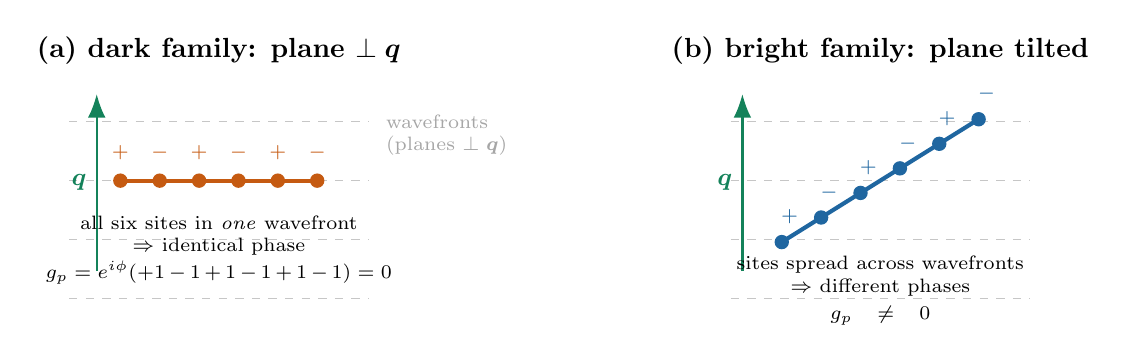
\begin{tikzpicture}[scale=1.0]

% ---------------- panel (a): dark hexagon ----------------
\begin{scope}
\node at (0,3.15) {\bfseries (a) dark family: plane $\perp\bq$};
% wavefronts
\foreach \y in {0,0.75,1.5,2.25}{
  \draw[gray!45,dashed] (-1.9,\y) -- (1.9,\y);
}
\node[gray!70,anchor=west,font=\scriptsize] at (2.0,2.25) {wavefronts};
\node[gray!70,anchor=west,font=\scriptsize] at (2.0,1.95)
     {(planes $\perp\bq$)};
% q arrow
\draw[-{Latex[length=3mm]},thick,acc] (-1.55,0.35) -- (-1.55,2.6)
   node[midway,left,font=\small]{$\bq$};
% hexagon seen edge-on, lying IN one wavefront
\draw[darkfam,line width=1.5pt] (-1.25,1.5) -- (1.25,1.5);
\foreach \x/\s in {-1.25/{+},-0.75/{-},-0.25/{+},0.25/{-},0.75/{+},1.25/{-}}{
  \fill[darkfam] (\x,1.5) circle (2.6pt);
  \node[font=\scriptsize,darkfam] at (\x,1.86) {$\s$};
}
\node[font=\scriptsize,align=center,text width=4.4cm] at (0,0.62)
  {all six sites in \emph{one} wavefront\\
   $\Rightarrow$ identical phase\\[2pt]
   $g_p=e^{i\phi}(+1-1+1-1+1-1)=0$};
\end{scope}

% ---------------- panel (b): bright hexagon ----------------
\begin{scope}[xshift=8.4cm]
\node at (0,3.15) {\bfseries (b) bright family: plane tilted};
\foreach \y in {0,0.75,1.5,2.25}{
  \draw[gray!45,dashed] (-1.9,\y) -- (1.9,\y);
}
\draw[-{Latex[length=3mm]},thick,acc] (-1.75,0.35) -- (-1.75,2.6)
   node[midway,left,font=\small]{$\bq$};
% tilted hexagon edge-on
\draw[brightfam,line width=1.5pt] (-1.25,0.72) -- (1.25,2.28);
\foreach \t/\s in {0/{+},0.2/{-},0.4/{+},0.6/{-},0.8/{+},1.0/{-}}{
  \pgfmathsetmacro{\xx}{-1.25+2.5*\t}
  \pgfmathsetmacro{\yy}{0.72+1.56*\t}
  \fill[brightfam] (\xx,\yy) circle (2.6pt);
  \node[font=\scriptsize,brightfam] at (\xx+0.10,\yy+0.32) {$\s$};
}
\node[font=\scriptsize,align=center,text width=4.6cm] at (0,0.10)
  {sites spread across wavefronts\\
   $\Rightarrow$ different phases\\[2pt]
   $g_p\neq0$};
\end{scope}

\end{tikzpicture}
\caption{The geometric origin of a dark family, drawn edge-on so that
wavefronts are lines. \textbf{(a)} When $\bq$ is parallel to a family's
$\langle111\rangle$ axis, that family's hexagons lie inside a single
wavefront. All six sites carry the same phase, the alternating signs
cancel in pairs, and $g_p$ vanishes identically. \textbf{(b)} Every
other family is tilted with respect to the wavefronts, its sites pick up
different phases, and $g_p\neq0$. At $L$ the measured geometric weights
$\sum_\mu|g^\mu_p|^2$ per family are $(96,96,\bm 0,96)$; the dark family
is exactly the one whose axis is parallel to $\bq$, with
$|\hat{\bm n}\cdot\hat{\bq}|=1.000000$.}
\label{fig:wavefront}
\end{figure}

\noindent
So at $L$ one quarter of all ring terms are \emph{blind} to the imposed
wave: flipping them changes the number the probe reads by exactly
nothing. We call that family \emph{dark}, and the other three
\emph{bright}. This is a statement about the momentum, not about any
state --- a point we return to in \S\ref{sec:state}.

\section{Dephasing: why bright plaquettes cost energy}

Now put the two ingredients together. Think of the excitation, to a
first approximation, as the ground state \emph{modulated} by the density
wave,
\begin{equation}
\psi(c)\;\simeq\;a(c)\,\psi_0(c).
\label{eq:modulated}
\end{equation}
This is the single-mode (Feynman) state $A_{\bq}|0\rangle$ written in
components. Ask what its ring coherence is on plaquette $p$. Coherence
is a sum over the pairs $(c,c')$ that $\Wp$ connects:
\begin{equation}
\langle\psi|\Wp|\psi\rangle
\;\sim\;\sum_{c\,\to\,c'}a^*(c')\,a(c)\,\psi_0(c')\,\psi_0(c).
\label{eq:coh}
\end{equation}
The ground state is stoquastic, so $\psi_0>0$ and every term in the
ground-state version of Eq.~(\ref{eq:coh}) adds constructively: that
positive interference \emph{is} the ground-state energy. In the excited
state each term is multiplied by $a^*(c')a(c)$, and by
Eq.~(\ref{eq:shift}) that factor depends entirely on whether $p$ is dark
or bright.

\begin{figure}[h]
\centering
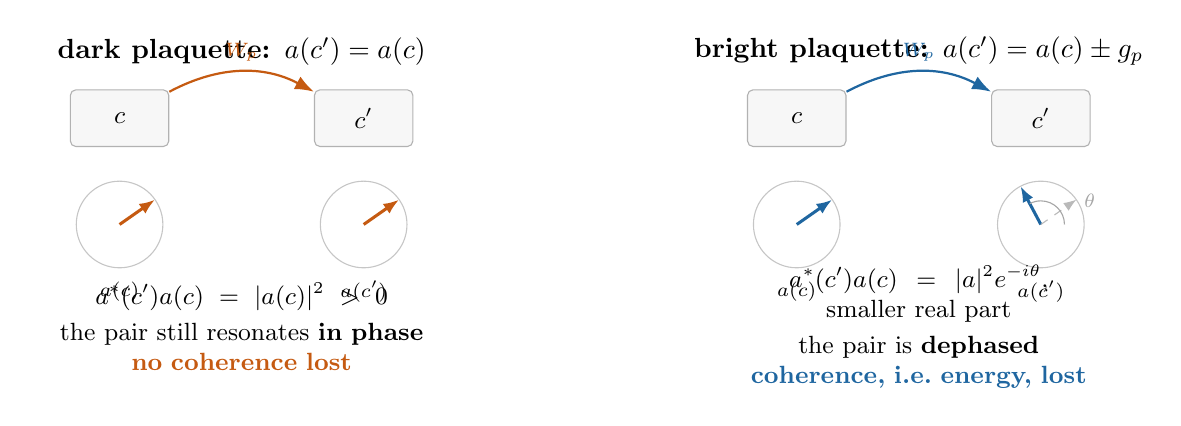
\begin{tikzpicture}[scale=1.0,
  cfg/.style={draw=gray!60,rounded corners=2pt,minimum width=1.25cm,
              minimum height=0.72cm,font=\small,fill=gray!6}]

% ------------- dark -------------
\begin{scope}
\node at (1.55,3.35) {\bfseries dark plaquette: $a(c')=a(c)$};
\node[cfg] (c1) at (0,2.5) {$c$};
\node[cfg] (c2) at (3.1,2.5) {$c'$};
\draw[-{Latex[length=2.4mm]},darkfam,thick]
  (c1) to[bend left=28] node[above,font=\scriptsize,darkfam]{$\Wp$} (c2);
% phasors
\begin{scope}[shift={(0,1.15)}]
  \draw[gray!45] (0,0) circle (0.55);
  \draw[-{Latex[length=2mm]},darkfam,line width=1.1pt]
     (0,0) -- (35:0.55);
  \node[font=\scriptsize] at (0,-0.85) {$a(c)$};
\end{scope}
\begin{scope}[shift={(3.1,1.15)}]
  \draw[gray!45] (0,0) circle (0.55);
  \draw[-{Latex[length=2mm]},darkfam,line width=1.1pt]
     (0,0) -- (35:0.55);
  \node[font=\scriptsize] at (0,-0.85) {$a(c')$};
\end{scope}
\node[font=\small,align=center,text width=5.2cm] at (1.55,-0.15)
  {$a^*(c')a(c)=|a(c)|^2>0$\\[2pt]
   the pair still resonates \textbf{in phase}\\
   \textcolor{darkfam}{\textbf{no coherence lost}}};
\end{scope}

% ------------- bright -------------
\begin{scope}[xshift=8.6cm]
\node at (1.55,3.35) {\bfseries bright plaquette: $a(c')=a(c)\pm g_p$};
\node[cfg] (d1) at (0,2.5) {$c$};
\node[cfg] (d2) at (3.1,2.5) {$c'$};
\draw[-{Latex[length=2.4mm]},brightfam,thick]
  (d1) to[bend left=28] node[above,font=\scriptsize,brightfam]{$\Wp$} (d2);
\begin{scope}[shift={(0,1.15)}]
  \draw[gray!45] (0,0) circle (0.55);
  \draw[-{Latex[length=2mm]},brightfam,line width=1.1pt]
     (0,0) -- (35:0.55);
  \node[font=\scriptsize] at (0,-0.85) {$a(c)$};
\end{scope}
\begin{scope}[shift={(3.1,1.15)}]
  \draw[gray!45] (0,0) circle (0.55);
  \draw[-{Latex[length=2mm]},brightfam,line width=1.1pt]
     (0,0) -- (118:0.55);
  \draw[-{Latex[length=1.6mm]},gray!55,dashed] (0,0) -- (35:0.55);
  \draw[gray!70] (0.30,0) arc (0:118:0.30);
  \node[font=\scriptsize,gray!70] at (0.62,0.30) {$\theta$};
  \node[font=\scriptsize] at (0,-0.85) {$a(c')$};
\end{scope}
\node[font=\small,align=center,text width=5.4cm] at (1.55,-0.15)
  {$a^*(c')a(c)=|a|^2e^{-i\theta}$, smaller real part\\[2pt]
   the pair is \textbf{dephased}\\
   \textcolor{brightfam}{\textbf{coherence, i.e.\ energy, lost}}};
\end{scope}

\end{tikzpicture}
\caption{The mechanism in one picture. A ring exchange connects two ice
configurations $c$ and $c'$. Each carries a phasor $a(c)$, the local
amplitude of the imposed density wave. On a \emph{dark} plaquette the
flip does not move the phasor at all, so the two configurations still
interfere constructively and the resonance survives untouched. On a
\emph{bright} plaquette the flip rotates the phasor by an amount set by
$g_p$, the interference is spoiled, and the lost coherence appears as
excitation energy.}
\label{fig:dephase}
\end{figure}

\noindent
This is also, finally, what the $f$-sum rule has been saying all along.
The exact first moment of the response is
\begin{equation}
f_1(\bq)=\frac{K}{2N}\sum_p\bigl\langle \Wp+\Wpd\bigr\rangle
\sum_\mu\bigl|g^\mu_p(\bq)\bigr|^2 ,
\label{eq:f1}
\end{equation}
a formula that had always looked like a geometric weight multiplying a
measured coherence. Equation~(\ref{eq:shift}) says what the weight
\emph{is}: $|g^\mu_p|^2$ is the dephasing that the imposed wave inflicts
on the ring resonance at $p$. The oscillator strength is the total
dephasing, and it is blind to the dark family because a dark plaquette
cannot be dephased.

\section{The bill, and where the relaxation happens}
\label{sec:state}

Everything so far concerns the \emph{momentum}: at $L$ a dark family
exists, and the rigid wave~(\ref{eq:modulated}) pays only on bright
plaquettes. That is not yet an explanation of why one eigenstate is soft
and its partner is not, because the dark family is equally available to
both. The distinction is what each state \emph{does} with it.

The rigid wave is a poor state and the true eigenstates relax away from
it. Reading the itemised bill off the exact eigenvectors --- projected
onto the state the probe actually creates at $\bq_L$, so that the answer
is basis-independent --- gives Table~\ref{tab:bill} and
Fig.~\ref{fig:ledger}.

\begin{table}[h]
\centering
\caption{Excitation energy in units of $K$ at $L$, $48$ sites, split by
whether the probe drives the family.}
\label{tab:bill}
\begin{tabular}{lccc}
\toprule
state & 3 bright families & 1 dark family & total\\
\midrule
rigid wave $A_{\bq}|0\rangle$ & $0.968$ & $0.878$ & $1.846$\\
\textbf{soft eigenstate}      & $\bm{0.108}$ & $0.915$ & $\bm{1.024}$\\
partner                       & $1.082$ & $0.648$ & $1.730$\\
\midrule
relaxation (rigid $\to$ soft) & $0.860$ \ (105\%) & $-0.038$ \ ($-5$\%)
 & $0.822$\\
\bottomrule
\end{tabular}
\end{table}

\begin{figure}[h]
\centering
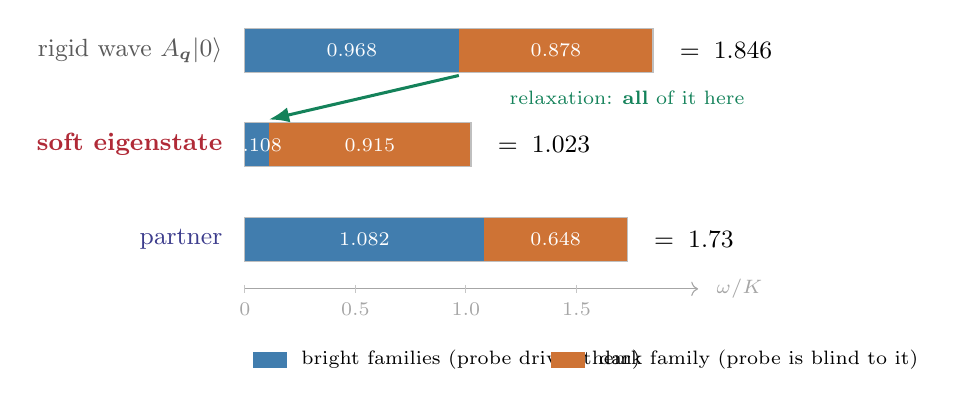
\begin{tikzpicture}[x=5.4cm,y=1cm]

\def\ymax{2.05}
% axis
\draw[->,gray!70] (0,-0.35) -- (\ymax*0.52,-0.35);
\foreach \v in {0,0.5,1.0,1.5}{
  \draw[gray!45] (\v*0.52,-0.30) -- (\v*0.52,-0.40)
     node[below,font=\scriptsize,gray!70]{$\v$};
}
\node[font=\scriptsize,gray!70,anchor=west] at (\ymax*0.52+0.02,-0.35)
  {$\omega/K$};

% bars: {y, bright, dark, label, colour}
\foreach \y/\b/\d/\lab/\col in {
   2.4/0.968/0.878/{rigid wave $A_{\bq}|0\rangle$}/gsc,
   1.2/0.108/0.915/{\textbf{soft eigenstate}}/softc,
   0.0/1.082/0.648/{partner}/phot}{
  \pgfmathsetmacro{\xb}{\b*0.52}
  \pgfmathsetmacro{\xt}{(\b+\d)*0.52}
  \pgfmathsetmacro{\tot}{\b+\d}
  \node[anchor=east,font=\small,\col] at (-0.03,\y+0.28) {\lab};
  \fill[brightfam!85] (0,\y) rectangle (\xb,\y+0.56);
  \fill[darkfam!85] (\xb,\y) rectangle (\xt,\y+0.56);
  \draw[gray!50] (0,\y) rectangle (\xt,\y+0.56);
  \node[font=\scriptsize,white] at (\xb/2,\y+0.28) {\b};
  \node[font=\scriptsize,white] at ({(\xb+\xt)/2},\y+0.28) {\d};
  \node[anchor=west,font=\small] at (\xt+0.04,\y+0.28)
    {$=\;\pgfmathprintnumber[fixed,precision=3]{\tot}$};
}

% relaxation arrow
\pgfmathsetmacro{\xa}{0.968*0.52}
\pgfmathsetmacro{\xc}{0.108*0.52}
\draw[-{Latex[length=2.6mm]},acc,line width=1.1pt]
  (\xa,2.36) -- (\xc,1.80);
\node[acc,font=\scriptsize,anchor=west] at (0.60,2.08)
  {relaxation: \textbf{all} of it here};

% legend
\fill[brightfam!85] (0.02,-1.35) rectangle (0.10,-1.15);
\node[anchor=west,font=\scriptsize] at (0.11,-1.25)
  {bright families (probe drives them)};
\fill[darkfam!85] (0.72,-1.35) rectangle (0.80,-1.15);
\node[anchor=west,font=\scriptsize] at (0.81,-1.25)
  {dark family (probe is blind to it)};

\end{tikzpicture}
\caption{The itemised energy bill at $L$. The rigid density wave pays
$0.968K$ of dephasing on the three bright families. The true soft
eigenstate has recovered almost all of it --- $0.968\to0.108$, an $89\%$
restoration --- while its dark-family cost is essentially unchanged.
\emph{The entire relaxation happens on the bright families.} The
partner, living in the orthogonal transverse channel, does not perform
this recovery and pays ten times more where the probe drives.}
\label{fig:ledger}
\end{figure}

\noindent
Read Fig.~\ref{fig:ledger} from the top down and the answer to ``why is
this state cheap?'' is immediate:

\begin{center}
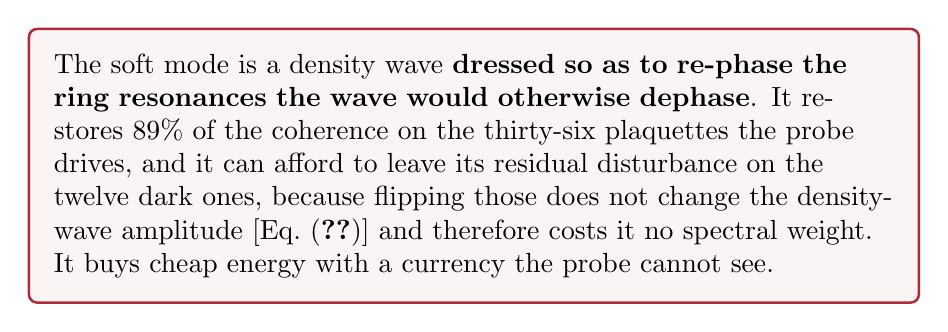
\begin{tikzpicture}
\node[draw=softc,line width=0.9pt,rounded corners=3pt,inner sep=9pt,
      fill=softc!5,text width=0.88\textwidth]{
The soft mode is a density wave \textbf{dressed so as to re-phase the
ring resonances the wave would otherwise dephase}. It restores $89\%$ of
the coherence on the thirty-six plaquettes the probe drives, and it can
afford to leave its residual disturbance on the twelve dark ones,
because flipping those does not change the density-wave amplitude
[Eq.~(\ref{eq:shift})] and therefore costs it no spectral weight. It
buys cheap energy with a currency the probe cannot see.};
\end{tikzpicture}
\end{center}

\noindent
That last clause is what makes the trade possible rather than merely
desirable. A state could always lower its energy by abandoning the
density wave --- but then it would no longer be created by the probe and
would carry no weight in $S^{zz}$. The dark family is the one place
where a state can rearrange itself \emph{without} paying that price.

\section{Why only at \texorpdfstring{$L$}{L}, and why only one of the two levels}

Two controls make the argument tight.

\paragraph{Momentum control ($X$).} At $X$ no $\langle111\rangle$ axis is
parallel to $\bq$, so no family is dark: the geometric weights are
$(96,96,96,96)$. There is nowhere to park the disturbance, the trade of
Fig.~\ref{fig:ledger} is unavailable, and nothing softens --- the lowest
$X$ level sits at $0.952$ of its Gaussian energy, against $0.503$ at
$L$. Softening tracks the \emph{existence} of a dark family.

\paragraph{State control (the partner).} At $L$ the dark family is
available to every level, yet only one exploits it. The soft mode pays
$0.108K$ on bright, the partner $1.082K$ --- a factor of ten, against an
overall energy ratio of only $0.59$. Availability is a property of the
momentum; exploitation is a property of the state. The same pattern
holds at $72$ sites, where the bright-family ratio is $0.282$ against an
overall ratio of $0.589$.

\section{A caveat that cost us a wrong figure}
\label{sec:caveat}

The sublattice label in Eq.~(\ref{eq:probe}) is not decoration. The
sublattice-\emph{summed} operator $A_{\bq}=\sum_\mu A^\mu_{\bq}$
commutes with \emph{every} ring exchange at $L$: its total alternating
sum vanishes on every hexagon, dark and bright alike. A check built on
that operator returns zero for both families and appears to confirm the
mechanism while actually testing nothing.

The correct statement uses the resolved operators, and it is stronger
than ``the total cancels'': on a dark plaquette
\emph{each} $g^\mu_p$ vanishes separately, so all four sublattice
amplitudes are individually unmoved by the flip. The cross-check is
that $\sum_\mu|g^\mu_p|^2$ summed over each family reproduces the
geometric weights $(96,96,0,96)$ exactly.

\section{The computed evidence}
\label{sec:evidence}

Everything above was asserted; this section is the arithmetic behind it.
All numbers come from exact diagonalization of the ground winding sector
of the $48$-site cluster fcc$(2,2,3)$ (dimension $9\,104$,
$E_0=-10.55601176\,K$) unless another size is named, and every script
that produced them is in the repository.

\paragraph{Gate.} The family decomposition used throughout must
reconstruct the Hamiltonian. It does:
$\sum_\mu\langle0|H_\mu|0\rangle=-10.5560117565$ against
$E_0=-10.5560117565$, a difference of $2.8\times10^{-14}$.

\subsection{The flip identity, Eq.~(\ref{eq:shift})}

For $4000$ ice configurations, every hexagon, every sublattice, we
flipped each flippable plaquette and compared the change in the
density-wave amplitude against $g^\mu_p$. The identity is exact
(Table~\ref{tab:flip}); note in particular that the dark family does not
merely have a small shift, it has none at all.

\begin{table}[h]
\centering
\caption{Direct verification of $a^\mu(c')-a^\mu(c)=\pm g^\mu_p$ at
$\bq_L$. The sign is per configuration (which way the ring flips).}
\label{tab:flip}
\begin{tabular}{ccccc}
\toprule
family $\mu$ & $n_{\rm hex}$ & $\max_\mu|g^\mu_p|$ &
$\max\bigl|\Delta a^\mu\mp g^\mu_p\bigr|$ & mean $|\Delta a^\mu|$\\
\midrule
$0$ & $12$ & $2.000000$ & $0.000\times10^{0}$ & $1.000000$\\
$1$ & $12$ & $2.000000$ & $0.000\times10^{0}$ & $1.000000$\\
\textbf{2 (dark)} & $12$ & $\bm{0.000000}$ & $0.000\times10^{0}$
 & $\bm{0.000000}$\\
$3$ & $12$ & $2.000000$ & $0.000\times10^{0}$ & $1.000000$\\
\bottomrule
\end{tabular}
\end{table}

\subsection{The dark family is the one whose axis is parallel to
\texorpdfstring{$\bq$}{q}}

Table~\ref{tab:geom} confirms the wavefront picture of
Fig.~\ref{fig:wavefront} quantitatively: the family with vanishing
geometric weight is precisely the family whose $\langle111\rangle$ axis
is parallel to $\bq_L$, to six digits.

\begin{table}[h]
\centering
\caption{Geometric weight $\sum_p\sum_\mu|g^\mu_p|^2$ per family at
$\bq_L=(\tfrac12,-\tfrac12,\tfrac12)$, against the orientation of each
family's axis.}
\label{tab:geom}
\begin{tabular}{ccccc}
\toprule
family $\mu$ & $n_{\rm hex}$ & $\sum|g|^2$ & $\langle111\rangle$ axis &
$|\hat{\bm n}\cdot\hat{\bq}|$\\
\midrule
$0$ & $12$ & $96.0000$ & $[1\,1\,1]$ & $0.333333$\\
$1$ & $12$ & $96.0000$ & $[1\,\bar1\,\bar1]$ & $0.333333$\\
\textbf{2 (dark)} & $12$ & $\bm{0.0000}$ & $[\bar1\,1\,\bar1]$ &
 $\bm{1.000000}$\\
$3$ & $12$ & $96.0000$ & $[\bar1\,\bar1\,1]$ & $0.333333$\\
\midrule
\multicolumn{5}{l}{\emph{at $X=(1,0,0)$:}\quad
$96.0,\;96.0,\;96.0,\;96.0$ \quad --- no family is dark}\\
\bottomrule
\end{tabular}
\end{table}

\noindent
The ground state does resonate on the dark family, so the cancellation
is not trivially about idle plaquettes: the family-resolved coherences
are $\langle\Wp+\Wpd\rangle_\mu=2.6296,\,3.2195,\,2.3535,\,2.3535$,
summing to $10.5560=|E_0|$. (They are unequal because the
$2\times2\times3$ box makes the four families inequivalent; this is a
finite-size effect, not physics.)

\subsection{The energy bill, and the two controls}

Table~\ref{tab:bill} in \S\ref{sec:state} gives the $48$-site ledger.
Table~\ref{tab:controls} adds what makes it an argument rather than an
observation.

\begin{table}[h]
\centering
\caption{Excitation energy in $K$, split by whether the probe drives the
family. The soft level's advantage is concentrated entirely in the
bright column; at $X$, where no family is dark, no such split exists and
nothing softens.}
\label{tab:controls}
\begin{tabular}{llccc c}
\toprule
& state & bright & dark & total & $\omega_{\rm low}/\omega_{\rm Gauss}$\\
\midrule
\multirow{2}{*}{48 sites, $L$}
 & soft    & $0.1081$ & $0.9154$ & $1.0235$ & $0.503$\\
 & partner & $1.0822$ & $0.6481$ & $1.7303$ & $0.851$\\
 & \emph{ratio} & $\bm{0.0999}$ & $1.4124$ & $0.5915$ &\\
\midrule
\multirow{2}{*}{72 sites, $L$}
 & soft    & $0.4585$ & $0.6095$ & $1.0681$ &\\
 & partner & $1.6237$ & $0.1906$ & $1.8143$ &\\
 & \emph{ratio} & $\bm{0.2824}$ & $3.1973$ & $0.5887$ &\\
\midrule
48 sites, $X$ & dominant & \multicolumn{2}{c}{no dark family exists}
 & $2.2354$ & $0.952$\\
\bottomrule
\end{tabular}
\end{table}

\noindent
Two things to read off. First, at both sizes the soft level's overall
advantage ($0.59$) is far smaller than its advantage on the driven
plaquettes ($0.10$ and $0.28$): the saving is specifically there, not
spread evenly. Second, at $X$ the trade is simply unavailable, and the
lowest level sits at $0.952$ of its Gaussian energy instead of $0.503$.
Softening tracks the \emph{existence} of a dark family.

\subsection{The consequence: a non-monotonic branch}

If the mechanism is right it should bend the dispersion, and it does.
Walking outward along $\Gamma\!\to\!L$, the branch rises like a photon,
turns over, and falls into the zone boundary
(Fig.~\ref{fig:disp}). Every cluster we can diagonalize shows it.

\begin{figure}[h]
\centering
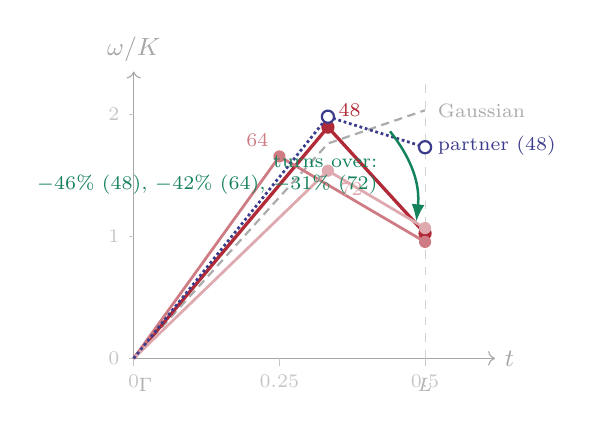
\begin{tikzpicture}[x=7.4cm,y=1.55cm]

% axes
\draw[->,gray!70] (0,0) -- (0.62,0) node[right,font=\small]{$t$};
\draw[->,gray!70] (0,0) -- (0,2.35) node[above,font=\small]{$\omega/K$};
\foreach \t in {0,0.25,0.5}{
  \draw[gray!45] (\t,0) -- (\t,-0.06) node[below,font=\scriptsize]{\t};
}
\foreach \w in {0,1,2}{
  \draw[gray!45] (0,\w) -- (-0.008,\w) node[left,font=\scriptsize]{\w};
}
\node[font=\scriptsize,gray!60] at (0.02,-0.22) {$\Gamma$};
\node[font=\scriptsize,gray!60] at (0.5,-0.22) {$L$};
\draw[gray!35,dashed] (0.5,0) -- (0.5,2.3);

% Gaussian reference: sigma 3.0 at t=1/3, 2sqrt3 at L, scale 0.58684
\draw[gray!65,dash pattern=on 3pt off 2pt,line width=0.8pt]
  (0,0) -- (0.3333,1.7605) -- (0.5,2.0333);
\node[gray!65,font=\scriptsize,anchor=west] at (0.505,2.03)
  {Gaussian};

% 48-site lower branch
\draw[softc,line width=1.2pt] (0,0) -- (0.3333,1.8949) -- (0.5,1.0235);
\foreach \t/\w in {0.3333/1.8949, 0.5/1.0235}{
  \fill[softc] (\t,\w) circle (2.4pt);}
\node[softc,font=\scriptsize,anchor=south west] at (0.335,1.90) {48};

% 64-site
\draw[softc!62,line width=1.0pt] (0,0) -- (0.25,1.6547) -- (0.5,0.9545);
\foreach \t/\w in {0.25/1.6547, 0.5/0.9545}{
  \fill[softc!62] (\t,\w) circle (2.2pt);}
\node[softc!62,font=\scriptsize,anchor=south east] at (0.248,1.66) {64};

% 72-site
\draw[softc!40,line width=1.0pt] (0,0) -- (0.3333,1.5380) -- (0.5,1.0681);
\foreach \t/\w in {0.3333/1.5380, 0.5/1.0681}{
  \fill[softc!40] (\t,\w) circle (2.2pt);}
\node[softc!40,font=\scriptsize,anchor=north west] at (0.338,1.52) {72};

% upper branch, 48
\draw[phot,line width=1.0pt,densely dotted]
  (0,0) -- (0.3333,1.9802) -- (0.5,1.7303);
\foreach \t/\w in {0.3333/1.9802, 0.5/1.7303}{
  \draw[phot,fill=white,line width=0.8pt] (\t,\w) circle (2.2pt);}
\node[phot,font=\scriptsize,anchor=west] at (0.505,1.74)
  {partner (48)};

% annotation
\draw[-{Latex[length=2.2mm]},acc,line width=0.9pt]
  (0.44,1.86) to[bend left=22] (0.485,1.12);
\node[acc,font=\scriptsize,anchor=east,align=right] at (0.435,1.50)
  {turns over:\\ $-46\%$ (48), $-42\%$ (64), $-31\%$ (72)};

\end{tikzpicture}
\caption{The lower branch along $\Gamma\to L$, with $\bq=t(1,\bar11)$.
It rises like a photon --- at $t=\tfrac13$ it is \emph{above} the
Gaussian curve, and nearly degenerate with its partner ($1.895$ against
$1.980$) --- then turns over and falls into the zone boundary. The
partner falls only $12.6\%$ over the same interval. Each cluster
resolves one interior momentum on this line, so what is established is
the inequality $\omega(\text{interior})>\omega(L)$ at three independent
sizes, not the shape of the minimum.}
\label{fig:disp}
\end{figure}

\subsection{What the ground state already knew}

Two ground-state quantities anticipate all of this, which is worth
recording because they are computable far beyond exact diagonalization.
The static structure factor is largest exactly where the mode softens
($S(L)=0.3704$, against $0.2872$, $0.2729$, $0.2583$, $0.1894$ at the
other resolved momenta), and the Feynman ratio $f_1/S$, normalized by
the Gaussian energy, orders all five momenta exactly as the measured
softening does --- Spearman correlation $+1$, no inversions.

\begin{table}[h]
\centering
\caption{The ground-state predictor against the measured softening. The
two right-hand columns rank the five momenta identically. Neither is
ordered by $|\bq|$: the first and last rows lie on the same shell.}
\label{tab:predict}
\begin{tabular}{lccccc}
\toprule
$\bq$ & $|\bq|$ & $S(\bq)$ & $f_1$ & $(f_1/S)/\omega_G$ &
$\omega_{\rm low}/\omega_G$\\
\midrule
$L$ & $0.866$ & $0.3704$ & $0.6835$ & $\bm{0.908}$ & $\bm{0.503}$\\
$(\frac13,\frac13,\frac23)$ & $0.816$ & $0.2870$ & $0.7150$ & $1.177$
 & $0.824$\\
$X$ & $1.000$ & $0.2727$ & $0.8790$ & $1.373$ & $0.952$\\
$(\frac13,\frac13,\frac13)$ & $0.577$ & $0.1894$ & $0.4585$ & $1.375$
 & $1.076$\\
$(\frac16,\frac16,\frac56)$ & $0.866$ & $0.2583$ & $0.8306$ & $1.415$
 & $1.114$\\
\bottomrule
\end{tabular}
\end{table}

\subsection{The baseline: no Gaussian theory can do this}

Finally, the reference the softening is measured against. In Gaussian
lattice electrodynamics the two transverse polarizations are not merely
close but \emph{exactly} degenerate: diagonalizing the lattice curl at
every allowed momentum of fcc$(4,4,4)$, fcc$(3,4,5)$ and fcc$(2,3,5)$
--- $153$ momenta in all, including $32$ in the generic class on the
anisotropic boxes --- gives $\sigma_2/\sigma_1=1.00000000$ every time,
with $\sigma_3/\sigma_1\sim10^{-15}$ confirming rank two.

Since $U$ and $K$ enter $\omega_\lambda=\sqrt{2UK}\,\sigma_\lambda$ only
through the common prefactor, \emph{no} renormalization of the Gaussian
theory --- of any strength, in either parameter --- can split the
doublet. The observed factor $1.69$ at $L$ is therefore outside that
description entirely, not a large correction within it.

\subsection{What this does not establish}
\label{sec:notclaimed}

Three things, stated so they are not read into the above.

\emph{This is not a new quasiparticle.} The soft level is one of the two
transverse polarizations, continuously connected to the photon doublet
at small $\bq$ (at $t=\tfrac13$ the two levels are $1.895$ and $1.980$,
nearly degenerate), carrying no new quantum number and no new
charge. What the mechanism describes is the \emph{same} excitation
reorganizing itself where the lattice permits --- which is exactly the
status of the roton in helium, where phonon and roton are one branch.

\emph{The minimum is not resolved.} Each cluster contributes one
interior point on the $\Gamma\to L$ line, so we establish
$\omega(\text{interior})>\omega(L)$ three times over, not the curvature
or position of a minimum.

\emph{The splitting itself is not new.} That interactions split the two
transverse polarizations at intermediate wavevector was predicted
semiclassically by Kwasigroch, Dou\c{c}ot and Castelnovo. What is added
here is that the splitting is order one at the zone boundary, that one
member falls to half the Gaussian energy while the other does not, and
the exact microscopic reason why.

\section{Summary}

\begin{enumerate}\setlength{\itemsep}{2pt}
\item Energy in this model \emph{is} ring coherence; an excitation is an
itemised bill over plaquettes.
\item In the ice basis the probe is diagonal, so a ring exchange either
shifts the density-wave amplitude or it does not:
$a^\mu(c')-a^\mu(c)=\pm g^\mu_p$, verified to $0.000\times10^{0}$.
\item Hexagons lying inside a wavefront have $g_p\equiv0$: they are
blind to the wave. At $L$ that is exactly one of the four families,
$25\%$ of all ring terms.
\item Dephasing is the energy: a flip that moves the phasor spoils the
constructive interference that made the ground state cheap. Hence
$f_1\propto\sum_p\langle \Wp+\Wpd\rangle|g_p|^2$ --- the oscillator
strength \emph{is} the total dephasing.
\item The rigid wave pays $0.968K$ of dephasing on bright plaquettes.
The true soft eigenstate recovers $89\%$ of it and parks the remainder
on the dark family, where rearrangement is free of spectral-weight cost.
Its partner does not, and pays ten times more.
\item No dark family, no softening: $X$ is the control.
\end{enumerate}

\end{document}
